\documentclass{standalone}
\usepackage{tikz}
\usetikzlibrary{patterns, positioning}

\begin{document}
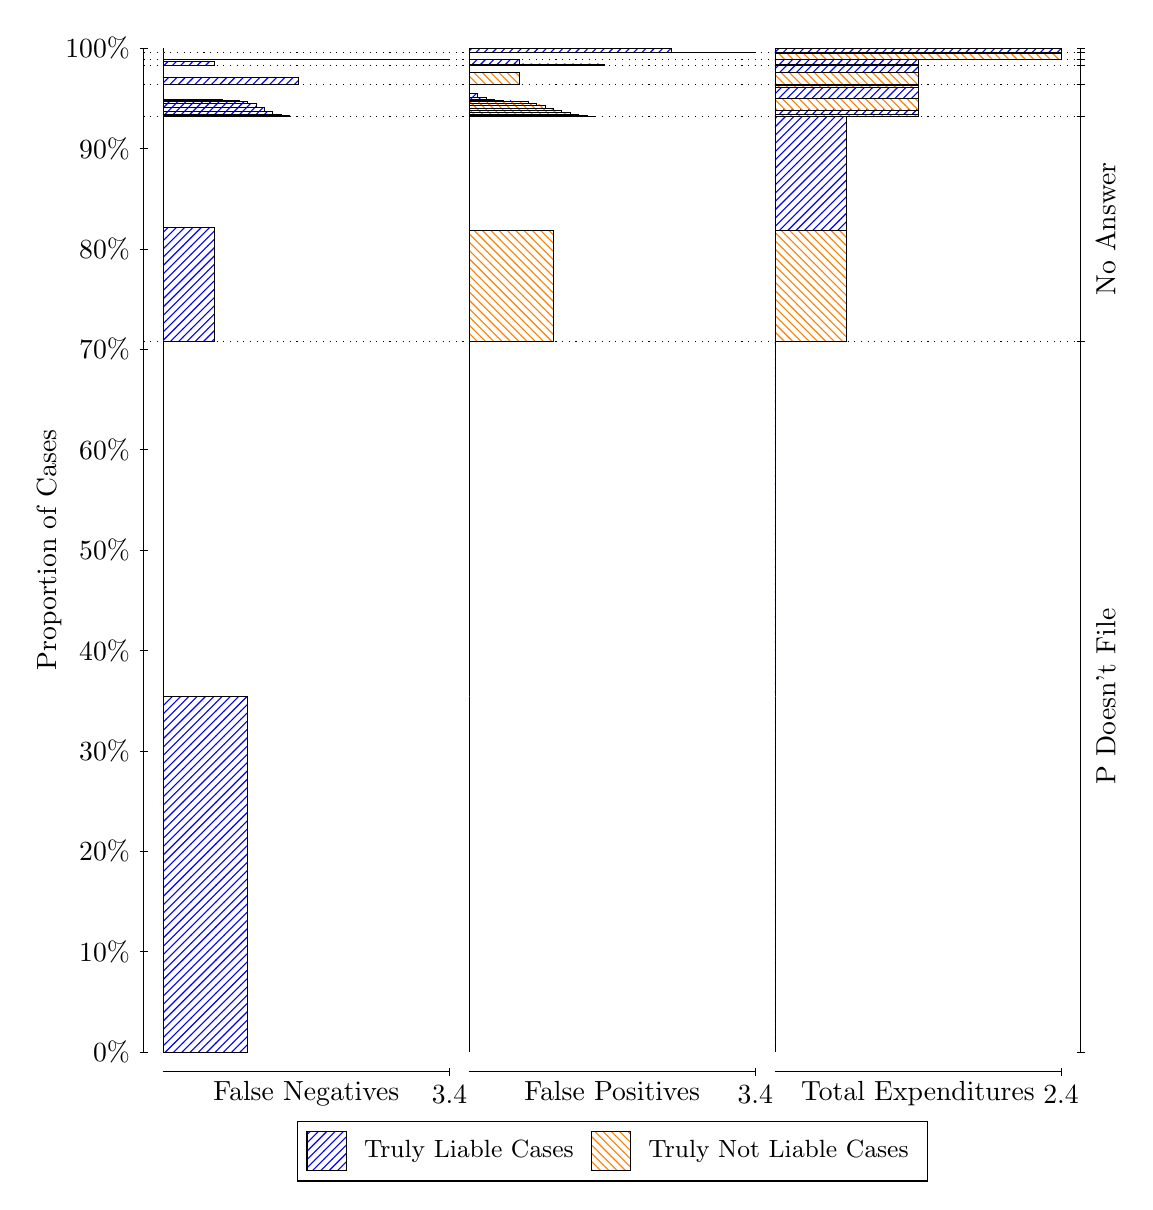
\begin{tikzpicture}
\draw[black, very thin] (1.5,1.75) -- (1.5,14.5);
\node[rotate=90, anchor=center] at (0.3, 8.125) {Proportion of Cases};
\draw[black, very thin] (1.45,1.75) -- (1.55,1.75);
\node[anchor=east] at (1.45, 1.75) {0\%};
\draw[black, very thin] (1.45,3.025) -- (1.55,3.025);
\node[anchor=east] at (1.45, 3.025) {10\%};
\draw[black, very thin] (1.45,4.3) -- (1.55,4.3);
\node[anchor=east] at (1.45, 4.3) {20\%};
\draw[black, very thin] (1.45,5.575) -- (1.55,5.575);
\node[anchor=east] at (1.45, 5.575) {30\%};
\draw[black, very thin] (1.45,6.85) -- (1.55,6.85);
\node[anchor=east] at (1.45, 6.85) {40\%};
\draw[black, very thin] (1.45,8.125) -- (1.55,8.125);
\node[anchor=east] at (1.45, 8.125) {50\%};
\draw[black, very thin] (1.45,9.4) -- (1.55,9.4);
\node[anchor=east] at (1.45, 9.4) {60\%};
\draw[black, very thin] (1.45,10.675) -- (1.55,10.675);
\node[anchor=east] at (1.45, 10.675) {70\%};
\draw[black, very thin] (1.45,11.95) -- (1.55,11.95);
\node[anchor=east] at (1.45, 11.95) {80\%};
\draw[black, very thin] (1.45,13.225) -- (1.55,13.225);
\node[anchor=east] at (1.45, 13.225) {90\%};
\draw[black, very thin] (1.45,14.5) -- (1.55,14.5);
\node[anchor=east] at (1.45, 14.5) {100\%};

\draw[black, very thin] (13.4,1.75) -- (13.4,14.5);
\draw[black, very thin] (13.35,1.75) -- (13.45,1.75);
\node[anchor=west] at (13.35, 1.75) {};
\draw[black, very thin] (13.35,10.777) -- (13.45,10.777);
\node[anchor=west] at (13.35, 10.777) {};
\draw[black, very thin] (13.35,13.627) -- (13.45,13.627);
\node[anchor=west] at (13.35, 13.627) {};
\draw[black, very thin] (13.35,14.042) -- (13.45,14.042);
\node[anchor=west] at (13.35, 14.042) {};
\draw[black, very thin] (13.35,14.275) -- (13.45,14.275);
\node[anchor=west] at (13.35, 14.275) {};
\draw[black, very thin] (13.35,14.354) -- (13.45,14.354);
\node[anchor=west] at (13.35, 14.354) {};
\draw[black, very thin] (13.35,14.442) -- (13.45,14.442);
\node[anchor=west] at (13.35, 14.442) {};
\draw[black, very thin] (13.35,14.5) -- (13.45,14.5);
\node[anchor=west] at (13.35, 14.5) {};

\draw[black, very thin, pattern color=blue, pattern=north east lines] (1.75,1.75) rectangle (2.8186,6.2636);
\draw[black, very thin, pattern color=orange, pattern=north west lines] (1.75,6.2636) rectangle (1.75,10.777);
\draw[black, very thin, pattern color=blue, pattern=north east lines] (1.75,10.777) rectangle (2.3912,12.224);
\draw[black, very thin, pattern color=orange, pattern=north west lines] (1.75,12.224) rectangle (1.75,13.627);
\draw[black, very thin, pattern color=blue, pattern=north east lines] (1.75,13.627) rectangle (3.3529,13.647);
\draw[black, very thin, pattern color=blue, pattern=north east lines] (1.75,13.647) rectangle (3.2461,13.655);
\draw[black, very thin, pattern color=blue, pattern=north east lines] (1.75,13.655) rectangle (3.1392,13.695);
\draw[black, very thin, pattern color=blue, pattern=north east lines] (1.75,13.695) rectangle (3.0324,13.745);
\draw[black, very thin, pattern color=blue, pattern=north east lines] (1.75,13.745) rectangle (2.9255,13.8);
\draw[black, very thin, pattern color=blue, pattern=north east lines] (1.75,13.8) rectangle (2.8186,13.819);
\draw[black, very thin, pattern color=blue, pattern=north east lines] (1.75,13.819) rectangle (2.7118,13.834);
\draw[black, very thin, pattern color=blue, pattern=north east lines] (1.75,13.834) rectangle (2.6049,13.839);
\draw[black, very thin, pattern color=blue, pattern=north east lines] (1.75,13.839) rectangle (2.498,13.845);
\draw[black, very thin, pattern color=orange, pattern=north west lines] (1.75,13.845) rectangle (1.75,14.042);
\draw[black, very thin, pattern color=blue, pattern=north east lines] (1.75,14.042) rectangle (3.4598,14.127);
\draw[black, very thin, pattern color=orange, pattern=north west lines] (1.75,14.127) rectangle (1.75,14.275);
\draw[black, very thin, pattern color=blue, pattern=north east lines] (1.75,14.275) rectangle (2.3912,14.33);
\draw[black, very thin, pattern color=orange, pattern=north west lines] (1.75,14.33) rectangle (1.75,14.354);
\draw[black, very thin, pattern color=blue, pattern=north east lines] (1.75,14.354) rectangle (5.3833,14.358);
\draw[black, very thin, pattern color=orange, pattern=north west lines] (1.75,14.358) rectangle (1.75,14.442);
\draw[black, very thin, pattern color=orange, pattern=north west lines] (1.75,14.442) rectangle (1.75,14.447);
\draw[black, very thin, pattern color=blue, pattern=north east lines] (1.75,14.447) rectangle (1.75,14.5);
\draw[black, very thin, pattern color=orange, pattern=north west lines] (5.6333,1.75) rectangle (5.6333,6.2637);
\draw[black, very thin, pattern color=blue, pattern=north east lines] (5.6333,6.2637) rectangle (5.6333,10.777);
\draw[black, very thin, pattern color=orange, pattern=north west lines] (5.6333,10.777) rectangle (6.702,12.181);
\draw[black, very thin, pattern color=blue, pattern=north east lines] (5.6333,12.181) rectangle (5.6333,13.627);
\draw[black, very thin, pattern color=orange, pattern=north west lines] (5.6333,13.627) rectangle (7.2363,13.634);
\draw[black, very thin, pattern color=orange, pattern=north west lines] (5.6333,13.634) rectangle (7.1294,13.64);
\draw[black, very thin, pattern color=orange, pattern=north west lines] (5.6333,13.64) rectangle (7.0225,13.655);
\draw[black, very thin, pattern color=orange, pattern=north west lines] (5.6333,13.655) rectangle (6.9157,13.679);
\draw[black, very thin, pattern color=orange, pattern=north west lines] (5.6333,13.679) rectangle (6.8088,13.711);
\draw[black, very thin, pattern color=orange, pattern=north west lines] (5.6333,13.711) rectangle (6.702,13.736);
\draw[black, very thin, pattern color=orange, pattern=north west lines] (5.6333,13.736) rectangle (6.5951,13.779);
\draw[black, very thin, pattern color=orange, pattern=north west lines] (5.6333,13.779) rectangle (6.4882,13.793);
\draw[black, very thin, pattern color=orange, pattern=north west lines] (5.6333,13.793) rectangle (6.3814,13.824);
\draw[black, very thin, pattern color=blue, pattern=north east lines] (5.6333,13.824) rectangle (6.1676,13.83);
\draw[black, very thin, pattern color=blue, pattern=north east lines] (5.6333,13.83) rectangle (6.0608,13.836);
\draw[black, very thin, pattern color=blue, pattern=north east lines] (5.6333,13.836) rectangle (5.9539,13.85);
\draw[black, very thin, pattern color=blue, pattern=north east lines] (5.6333,13.85) rectangle (5.8471,13.87);
\draw[black, very thin, pattern color=blue, pattern=north east lines] (5.6333,13.87) rectangle (5.7402,13.924);
\draw[black, very thin, pattern color=blue, pattern=north east lines] (5.6333,13.924) rectangle (5.6333,14.042);
\draw[black, very thin, pattern color=orange, pattern=north west lines] (5.6333,14.042) rectangle (6.2745,14.19);
\draw[black, very thin, pattern color=blue, pattern=north east lines] (5.6333,14.19) rectangle (5.6333,14.275);
\draw[black, very thin, pattern color=orange, pattern=north west lines] (5.6333,14.275) rectangle (7.3431,14.299);
\draw[black, very thin, pattern color=blue, pattern=north east lines] (5.6333,14.299) rectangle (6.2745,14.354);
\draw[black, very thin, pattern color=orange, pattern=north west lines] (5.6333,14.354) rectangle (5.6333,14.438);
\draw[black, very thin, pattern color=blue, pattern=north east lines] (5.6333,14.438) rectangle (5.6333,14.442);
\draw[black, very thin, pattern color=orange, pattern=north west lines] (5.6333,14.442) rectangle (9.2667,14.447);
\draw[black, very thin, pattern color=blue, pattern=north east lines] (5.6333,14.447) rectangle (8.198,14.5);
\draw[black, very thin, pattern color=orange, pattern=north west lines] (9.5167,1.75) rectangle (9.5167,6.2637);
\draw[black, very thin, pattern color=blue, pattern=north east lines] (9.5167,6.2637) rectangle (9.5167,10.777);
\draw[black, very thin, pattern color=orange, pattern=north west lines] (9.5167,10.777) rectangle (10.425,12.181);
\draw[black, very thin, pattern color=blue, pattern=north east lines] (9.5167,12.181) rectangle (10.425,13.627);
\draw[black, very thin, pattern color=orange, pattern=north west lines] (9.5167,13.627) rectangle (11.333,13.66);
\draw[black, very thin, pattern color=blue, pattern=north east lines] (9.5167,13.66) rectangle (11.333,13.714);
\draw[black, very thin, pattern color=orange, pattern=north west lines] (9.5167,13.714) rectangle (11.333,13.857);
\draw[black, very thin, pattern color=blue, pattern=north east lines] (9.5167,13.857) rectangle (11.333,14);
\draw[black, very thin, pattern color=orange, pattern=north west lines] (9.5167,14) rectangle (11.333,14.021);
\draw[black, very thin, pattern color=blue, pattern=north east lines] (9.5167,14.021) rectangle (11.333,14.042);
\draw[black, very thin, pattern color=orange, pattern=north west lines] (9.5167,14.042) rectangle (11.333,14.19);
\draw[black, very thin, pattern color=blue, pattern=north east lines] (9.5167,14.19) rectangle (11.333,14.275);
\draw[black, very thin, pattern color=orange, pattern=north west lines] (9.5167,14.275) rectangle (11.333,14.299);
\draw[black, very thin, pattern color=blue, pattern=north east lines] (9.5167,14.299) rectangle (11.333,14.354);
\draw[black, very thin, pattern color=orange, pattern=north west lines] (9.5167,14.354) rectangle (13.15,14.438);
\draw[black, very thin, pattern color=blue, pattern=north east lines] (9.5167,14.438) rectangle (13.15,14.442);
\draw[black, very thin, pattern color=orange, pattern=north west lines] (9.5167,14.442) rectangle (13.15,14.447);
\draw[black, very thin, pattern color=blue, pattern=north east lines] (9.5167,14.447) rectangle (13.15,14.5);
\draw[black, dotted] (1.5,10.777) -- (13.4,10.777);
\draw[black, dotted] (1.5,13.627) -- (13.4,13.627);
\draw[black, dotted] (1.5,14.042) -- (13.4,14.042);
\draw[black, dotted] (1.5,14.275) -- (13.4,14.275);
\draw[black, dotted] (1.5,14.354) -- (13.4,14.354);
\draw[black, dotted] (1.5,14.442) -- (13.4,14.442);
\draw[black, very thin] (1.75,1.5) -- (5.3833,1.5);
\node[anchor=north] at (3.5667, 1.5) {False Negatives};
\draw[black, very thin] (5.3833,1.45) -- (5.3833,1.55);
\node[anchor=north] at (5.3833, 1.45) {3.4};

\draw[black, very thin] (5.6333,1.5) -- (9.2667,1.5);
\node[anchor=north] at (7.45, 1.5) {False Positives};
\draw[black, very thin] (9.2667,1.45) -- (9.2667,1.55);
\node[anchor=north] at (9.2667, 1.45) {3.4};

\draw[black, very thin] (9.5167,1.5) -- (13.15,1.5);
\node[anchor=north] at (11.333, 1.5) {Total Expenditures};
\draw[black, very thin] (13.15,1.45) -- (13.15,1.55);
\node[anchor=north] at (13.15, 1.45) {2.4};

\node[black, centered, rotate=90] at (13.72, 6.2636) {P Doesn't File};
\node[black, centered, rotate=90] at (13.72, 12.202) {No Answer};






\draw (7.449999999999999,1.5) node[draw=none] (baseCoordinate) {};
\begin{scope}[align=center]
        \matrix[scale=0.5, draw=black, below=0.5cm of baseCoordinate, nodes={draw}, column sep=0.1cm]{
            \node[rectangle, draw, minimum width=0.5cm, minimum height=0.5cm, pattern=north east lines, pattern color=blue] {}; &
            \node[draw=none, font=\small] (B) {Truly Liable Cases}; &
            \node[rectangle, draw, minimum width=0.5cm, minimum height=0.5cm, pattern=north west lines, pattern color=orange] {}; &
            \node[draw=none, font=\small] (B) {Truly Not Liable Cases}; \\
            };
\end{scope}

\end{tikzpicture}
\end{document}